% Options for packages loaded elsewhere
\PassOptionsToPackage{unicode}{hyperref}
\PassOptionsToPackage{hyphens}{url}
%
\documentclass[
  english,
  man]{apa6}
\usepackage{lmodern}
\usepackage{amssymb,amsmath}
\usepackage{ifxetex,ifluatex}
\ifnum 0\ifxetex 1\fi\ifluatex 1\fi=0 % if pdftex
  \usepackage[T1]{fontenc}
  \usepackage[utf8]{inputenc}
  \usepackage{textcomp} % provide euro and other symbols
\else % if luatex or xetex
  \usepackage{unicode-math}
  \defaultfontfeatures{Scale=MatchLowercase}
  \defaultfontfeatures[\rmfamily]{Ligatures=TeX,Scale=1}
\fi
% Use upquote if available, for straight quotes in verbatim environments
\IfFileExists{upquote.sty}{\usepackage{upquote}}{}
\IfFileExists{microtype.sty}{% use microtype if available
  \usepackage[]{microtype}
  \UseMicrotypeSet[protrusion]{basicmath} % disable protrusion for tt fonts
}{}
\makeatletter
\@ifundefined{KOMAClassName}{% if non-KOMA class
  \IfFileExists{parskip.sty}{%
    \usepackage{parskip}
  }{% else
    \setlength{\parindent}{0pt}
    \setlength{\parskip}{6pt plus 2pt minus 1pt}}
}{% if KOMA class
  \KOMAoptions{parskip=half}}
\makeatother
\usepackage{xcolor}
\IfFileExists{xurl.sty}{\usepackage{xurl}}{} % add URL line breaks if available
\IfFileExists{bookmark.sty}{\usepackage{bookmark}}{\usepackage{hyperref}}
\hypersetup{
  pdftitle={Metodologi Penelitian dalam Psikologi Politik},
  hidelinks,
  pdfcreator={LaTeX via pandoc}}
\urlstyle{same} % disable monospaced font for URLs
\usepackage{graphicx,grffile}
\makeatletter
\def\maxwidth{\ifdim\Gin@nat@width>\linewidth\linewidth\else\Gin@nat@width\fi}
\def\maxheight{\ifdim\Gin@nat@height>\textheight\textheight\else\Gin@nat@height\fi}
\makeatother
% Scale images if necessary, so that they will not overflow the page
% margins by default, and it is still possible to overwrite the defaults
% using explicit options in \includegraphics[width, height, ...]{}
\setkeys{Gin}{width=\maxwidth,height=\maxheight,keepaspectratio}
% Set default figure placement to htbp
\makeatletter
\def\fps@figure{htbp}
\makeatother
\setlength{\emergencystretch}{3em} % prevent overfull lines
\providecommand{\tightlist}{%
  \setlength{\itemsep}{0pt}\setlength{\parskip}{0pt}}
\setcounter{secnumdepth}{-\maxdimen} % remove section numbering
% Manuscript styling
\usepackage{csquotes}
\usepackage{upgreek}
\captionsetup{font=singlespacing,justification=justified}

% Table formatting
\usepackage{longtable}
\usepackage{lscape}
% \usepackage[counterclockwise]{rotating}   % Landscape page setup for large tables
\usepackage{multirow}		% Table styling
\usepackage{tabularx}		% Control Column width
\usepackage[flushleft]{threeparttable}	% Allows for three part tables with a specified notes section
\usepackage{threeparttablex}            % Lets threeparttable work with longtable

% Create new environments so endfloat can handle them
% \newenvironment{ltable}
%   {\begin{landscape}\begin{center}\begin{threeparttable}}
%   {\end{threeparttable}\end{center}\end{landscape}}
\newenvironment{lltable}{\begin{landscape}\begin{center}\begin{ThreePartTable}}{\end{ThreePartTable}\end{center}\end{landscape}}

% Enables adjusting longtable caption width to table width
% Solution found at http://golatex.de/longtable-mit-caption-so-breit-wie-die-tabelle-t15767.html
\makeatletter
\newcommand\LastLTentrywidth{1em}
\newlength\longtablewidth
\setlength{\longtablewidth}{1in}
\newcommand{\getlongtablewidth}{\begingroup \ifcsname LT@\roman{LT@tables}\endcsname \global\longtablewidth=0pt \renewcommand{\LT@entry}[2]{\global\advance\longtablewidth by ##2\relax\gdef\LastLTentrywidth{##2}}\@nameuse{LT@\roman{LT@tables}} \fi \endgroup}

% \setlength{\parindent}{0.5in}
% \setlength{\parskip}{0pt plus 0pt minus 0pt}

% Overwrite redefinition of paragraph and subparagraph by the default LaTeX template
% See https://github.com/crsh/papaja/issues/292
\makeatletter
\renewcommand{\paragraph}{\@startsection{paragraph}{4}{\parindent}%
  {0\baselineskip \@plus 0.2ex \@minus 0.2ex}%
  {-1em}%
  {\normalfont\normalsize\bfseries\itshape\typesectitle}}

\renewcommand{\subparagraph}[1]{\@startsection{subparagraph}{5}{1em}%
  {0\baselineskip \@plus 0.2ex \@minus 0.2ex}%
  {-\z@\relax}%
  {\normalfont\normalsize\itshape\hspace{\parindent}{#1}\textit{\addperi}}{\relax}}
\makeatother

% \usepackage{etoolbox}
\makeatletter
\patchcmd{\HyOrg@maketitle}
  {\section{\normalfont\normalsize\abstractname}}
  {\section*{\normalfont\normalsize\abstractname}}
  {}{\typeout{Failed to patch abstract.}}
\makeatother
\shorttitle{Metodologi Penelitian dalam Psikologi Politik}
\author{Rizqy Amelia Zein\textsuperscript{1,2}}
\affiliation{
\vspace{0.5cm}
\textsuperscript{1} Departemen Psikologi Kepribadian dan Sosial, Fakultas Psikologi Universitas Airlangga\\\textsuperscript{2} Institute for Globally Distributed Open Research and Education (IGDORE)}
\authornote{Naskah ini ditulis untuk diajukan sebagai bagian dari buku teks **Pengantar Psikologi Politik** yang diterbitkan oleh Ikatan Psikologi Sosial.


Correspondence concerning this article should be addressed to Rizqy Amelia Zein, Kampus B Universitas Airlangga, Jalan Airlangga 4-6 Surabaya, Jawa Timur 60286. E-mail: amelia.zein@psikologi.unair.ac.id}
\DeclareDelayedFloatFlavor{ThreePartTable}{table}
\DeclareDelayedFloatFlavor{lltable}{table}
\DeclareDelayedFloatFlavor*{longtable}{table}
\makeatletter
\renewcommand{\efloat@iwrite}[1]{\immediate\expandafter\protected@write\csname efloat@post#1\endcsname{}}
\makeatother
\usepackage{lineno}

\linenumbers
\usepackage[titles]{tocloft}
\cftpagenumbersoff{figure}
\renewcommand{\cftfigpresnum}{\itshape\figurename\enspace}
\renewcommand{\cftfigaftersnum}{.\space}
\setlength{\cftfigindent}{0pt}
\setlength{\cftafterloftitleskip}{0pt}
\settowidth{\cftfignumwidth}{Figure 10.\qquad}
\ifxetex
  % Load polyglossia as late as possible: uses bidi with RTL langages (e.g. Hebrew, Arabic)
  \usepackage{polyglossia}
  \setmainlanguage[]{english}
\else
  \usepackage[shorthands=off,main=english]{babel}
\fi

\title{Metodologi Penelitian dalam Psikologi Politik}

\date{}

\begin{document}
\maketitle

Meskipun hitung cepat (\emph{quick count}) mayoritas lembaga survei menunjukkan temuan yang bertolak belakang, Prabowo Subianto, calon Presiden pada Pemilihan Umum (Pemilu) 2019, buru-buru mengumumkan kemenangannya di depan awak media beberapa jam setelah Tempat Pemungutan Suara (TPS) ditutup. Berbekal temuan hitung cepat dan \emph{exit poll} dari beberapa lembaga survei sekaligus perhitungan riil (\emph{real count}) yang dilakukan oleh relawannya, Prabowo mengumumkan setidaknya ia meraup suara dengan margin yang sangat besar. Meskipun temuan lembaga survei yang dirujuk Prabowo bertolak belakang dengan kebanyakan lembaga survei termasuk perhitungan resmi Komisi Pemilihan Umum (KPU), Prabowo dan pendukungnya amat mempercayai temuan lembaga survei yang memenangkan Prabowo dan dengan lantang menuduh lembaga survei yang berbeda dengan klaimnya merupakan lembaga bayaran, tidak saintifik, dan partisan.

Dari kasus diatas tentu menarik untuk membahas pertanyaan-pertanyaan seperti; bagaimana sebenarnya cara terbaik untuk membedakan informasi yang saintifik, sains semu (\emph{pseudoscience}), mis/disinformasi, dan khayalan? Bagaimana sesungguhnya cara kerja ilmuwan dalam menghasilkan temuan yang saintifik? Dan bagaimana seharusnya temuan penelitian dilaporkan dan disebarluaskan?

\hypertarget{logika-saintifik-scientific-reasoning}{%
\subsection{\texorpdfstring{1. Logika saintifik (\emph{scientific reasoning})}{1. Logika saintifik (scientific reasoning)}}\label{logika-saintifik-scientific-reasoning}}

Apabila anda mengingat kembali berbagai konsep yang telah anda pelajari di mata kuliah Pengantar Psikologi, anda mendapati hal-hal yang menarik, seperti; anak-anak dapat menirukan perilaku kekerasan (yaitu dengan memukul boneka Bobo) dengan mengamati orang dewasa yang melakukan perilaku tersebut, atau pembalap sepeda meraih waktu tempuh yang lebih cepat ketika membalap bersama orang lain daripada mengendarai sepedanya sendirian. Atau anda mungkin masih mengingat studi Latane dan Darley yang sangat populer, yang menunjukkan bahwa semakin banyak orang mendapati keadaan darurat, dimana seorang korban membutuhkan bantuan, justru menurunkan peluang korban tersebut mendapatkan bantuan. Mungkin anda juga bertanya-tanya mengapa anda tidak diajarkan cara membaca karakter seseorang dari garis tangan atau sidik jarinya, meskipun teknik ini sangat populer di kalangan awam.

Teori-teori di Psikologi pada dasarnya dibangun dengan pengamatan yang cermat dan sistematis, bukan yang ceroboh dan mengandalkan intuisi. Ilmuwan Psikologi tidak boleh menebak-nebak atau mencocok-cocokkan antara satu kejadian dengan kejadian yang lain. Untuk mengetahui apa yang bisa dan tidak bisa dipercaya, ilmuwan Psikologi sangat mengandalkan pengamatan yang cermat. Meskipun ada beberapa pendekatan yang menawarkan cara alternatif dalam merumuskan pengetahuan, pendekatan \emph{empirisme} adalah yang paling dominan di sejarah perkembangan ilmu Psikologi.

Persoalan membedakan antara yang saintifik dengan yang tidak merupakan problem klasik yang diperdebatkan para filosof sejak dulu. Karl Popper (1902-1994) merupakan salah satu filosof yang cukup cerdik mengartikulasikan permasalahan ini dengan menyebutnya \textbf{problem demarkasi}. Popper sebenarnya tidak terlalu tertarik untuk memberikan label atas \enquote{mana yang saintifik dan yang tidak}, namun ia lebih banyak menjelaskan bagaimana strategi terbaik untuk menghasilkan pengetahuan yang saintifik.

Awalnya, filosof positivis percaya bahwa satu-satunya cara yang ampuh dalam memisahkan antara yang saintifik dengan yang tidak adalah dengan melakukan \emph{verifikasi}. Prosedur ini dilakukan peneliti dengan memeriksa kesesuaian antara asumsi, teori, atau hipotesis dengan bukti empirik. Apabila bukti empirik yang tersedia konsisten dengan pernyataan yang hendak diuji, maka pernyataan tersebut dinyatakan terbukti sehingga dianggap saintifik.

Sebelum dicari korespondensinya pada realitas yang sedang diamati, pernyataan yang akan diuji harus memiliki \textbf{kriteria verifikasi} yang artinya, suatu teori \textbf{hanya dapat diverifikasi} ketika peneliti dapat menjelaskan secara rinci bagaimana langkah-langkah pengujiannya dalam bentuk \textbf{definisi operasional}. Definisi operasional adalah deskripsi yang memuat prosedur rinci yang harus dilakukan pengamat dalam menentukan eksistensi (ada/tidaknya) dan kualitas fenomena atau konsep yang diamati (Dienes, 2008).

Filosof yang mendukung positivisme tidak menyadari bahwa ada problem yang amat mendasar dari prosedur verifikasi. Utamanya ketika memastikan apakah bukti empirik yang diperoleh dari satu pengamatan akan berlaku pada pengamatan yang lain. Misalnya, ketika Ngadiman mengetahui bahwa (1) cabai berwarna merah, apakah (2) semua cabai akan memiliki warna yang sama? Pernyataan (1) dapat diperiksa melalui pengamatan langsung dengan logika \textbf{deduksi}, sedangkan permasalahan pada pernyataan (2) dapat diselesaikan dengan logika \textbf{induksi}.

\textbf{Deduksi} merupakan proses penarikan kesimpulan yang mengandaikan apabila terdapat hubungan yang logis antara dua pernyataan, maka kesimpulan yang mengikutinya akan sahih pula. Misalnya,

\begin{enumerate}
\def\labelenumi{\arabic{enumi}.}
\tightlist
\item
  Semua cabai berwarna merah
\item
  Ngadiman memetik cabai
\end{enumerate}

\textbf{Maka: Cabai Ngadiman berwarna merah}

Sedangkan induksi merupakan proses penarikan kesimpulan dari pengamatan berulang atas suatu gejala, misalnya

\begin{enumerate}
\def\labelenumi{\arabic{enumi}.}
\tightlist
\item
  Ngadiman memetik cabai berwarna merah
\item
  Yuli memetik cabai berwarna merah
\item
  Sunu memetik cabai berwarna merah
\item
  Bejo memetik cabai berwarna merah
\item
  Dono memetik cabai berwarna merah
\end{enumerate}

\textbf{Maka: semua cabai berwarna merah}

Kesimpulan dari logika induksi di atas tentu tak bisa serta-merta dianggap benar, sedangkan kesimpulan yang ditarik dengan logika deduksi juga sangat dangkal. Bagaimana mungkin dengan hanya satu kali mengamati, Ngadiman dapat yakin bahwa teorinya (semua cabai berwarna merah) tepat? Di sisi lain, meskipun Ngadiman tidak lagi sendirian mengamati warna cabai, rasanya janggal apabila kita langsung meyakini bahwa semua cabai berwarna merah. Namun tentu saja, apabila kita terus-menerus mendapati bukti yang konsisten setelah berulang kali mengamati, kita akan lebih percaya diri dalam menarik kesimpulan. Oleh karena itu, dapat disimpulkan bahwa kemungkinan kesimpulan pengamatan berlaku secara umum (generalisasi) akan meningkat seiring dengan ditemukannya bukti yang mendukung, ketika mengamatinya berulang-ulang.

Manariknya, Popper menolak asumsi ini. Klaim bahwa suatu pernyataan dapat dikatakan benar ketika bukti yang konsisten terakumulasi dari pengamatan berulang adalah sesuatu yang tidak masuk akal. Ketika kita akan mengamati warna cabai, tidak ada jaminan bahwa kita akan mendapati warna yang sama dengan pengamatan kita sebelumnya. Kita juga tidak bisa memperkirakan seberapa mungkin temuan kita sebelumnya, akan kita temui lagi di pengamatan berikutnya. Yang terpenting dari kritik Popper pada filosof positivisme adalah ketika mengasumsikan suatu teori adalah benar, sesungguhnya secara paradoks kita sekaligus mengasumsikan bahwa teori tersebut salah. Oleh karena itu, \textbf{suatu teori hanya akan benar selama tidak ada bukti yang dapat menggugurkannya}. Pernyataan \emph{semua cabai berwana merah} akan langsung gugur apabila seorang pengamat menemukan ada \emph{satu cabai yang berwarna hijau}. Popper menyebutkan bahwa pengetahuan saintifik tidak mungkin didapatkan dengan sekadar mengamati gejala. Merumuskan teori sesungguhnya bukan tujuan sains, karena kepastian dan kebenaran mutlak dari suatu teori tak mungkin dapat dicapai. Popper juga menunjukkan bahaya \emph{fallibilism}, yaitu amat mungkin hal-hal yang kita percayai justru sesungguhnya sangat keliru.

Sepanjang sejarah sains, kita sering menemukan episode dimana sekelompok orang berusaha mempertahankan tradisi mengenai \enquote{apa-apa yang sudah kadung mereka percayai} sehingga penyimpangan atas tradisi ini berakibat pengucilan dan pembungkaman. Sebaliknya, sains justru berkembang dalam situasi yang penuh kontradiksi - ketika bukti baru, teknik baru, temuan baru, tokoh baru, menantang kepercayaan yang sudah mapan. Popper dengan tegas mengusulkan bahwa tujuan sains seharusnya adalah \textbf{memfalsifikasi}, yaitu mencari bukti yang bertentangan dengan keyakinan atau asumsi yang dimiliki oleh peneliti (Thornton, 2019). Apabila peneliti menemukan bukti mendukung teorinya, maka \textbf{bukan berarti} teori tersebut benar atau terbukti benar (\emph{proved/established}), tetapi peneliti hanya dapat mengklaim bahwa teorinya \textbf{didukung oleh bukti} (\emph{corroborated}). Teori tersebut berhasil dipertahankan dengan pengujian yang cermat melalui proses falsifikasi, bukan karena ia \enquote{mutlak benar}, namun karena \enquote{sementara ini} teori tersebut yang paling mendekati kebenaran. Premis inilah yang kemudian menjadi sifat dasar sains, yaitu kesementaraan (provisional). Dengan kata lain, teori hanya dapat dianggap benar selama belum ada bukti yang menggugurkannya. Seiring dengan munculnya teknik baru, cara baru, dan bukti baru yang menambal kekurangan penelitian sebelumnya, maka pemahaman kita atas realitas akan semakin berkembang. Oleh karena itu, selain membutuhkan kebaruan dan inovasi, sains juga membutuhkan koreksi atas dirinya sendiri (\emph{self-correction}) (Nosek et al., 2015).

\hypertarget{strategi-pemeriksaan-kredibilitas-temuan-penelitian}{%
\subsection{2. Strategi pemeriksaan kredibilitas temuan penelitian}\label{strategi-pemeriksaan-kredibilitas-temuan-penelitian}}

Sebagai mahasiswa Psikologi, tentu anda diwajibkan untuk mengerjakan proyek penelitian secara mandiri kemudian menulis laporan tugas akhir agar dapat dinyatakan lulus. Sebagian dari anda mungkin memiliki aspirasi untuk menjadi peneliti atau dosen di perguruan tinggi sebagai pilihan karir. Ada yang mungkin berkeingingan menjadi ilmuwan data (\emph{data scientist}) yang banyak bersentuhan dengan \emph{data mining} dan dataset skala besar untuk dianalisis. Dalam konteks ini, anda adalah \emph{pelaku} penelitian - dimana anda banyak berperan dalam merumuskan pertanyaan penelitian, mendesain studi yang ditujukan untuk menjawab pertanyaan tersebut, melakukan pengambilan data, menganalisisnya, lalu melaporkan, dan mengkomunikasikan temuan pada khalayak yang lebih luas.

Sedangkan sebagian dari anda mungkin lebih tertarik menjadi praktisi - misalnya, bekerja sebagai manajer tim kampanye, atau sebagai konsultan politik. Sebagian mungkin tertarik bekerja di perusahaan media, atau mungkin bekerja sebagai tim ahli di parlemen atau di kantor pemerintah lainnya. Sebagian yang lain mungkin tertarik menjadi konselor bagi calon anggota dewan yang gagal terpilih. Dalam konteks ini, dalam mengerjakan pekerjaan anda sehari-hari, anda dituntut untuk mengambil keputusan yang \textbf{berbasis bukti} - yaitu, informasi yang didukung sehingga menjadi anda diharuskan menjadi \emph{pengguna} hasil penelitian (Morling, 2018).

Pada praktiknya, anda melakukan kedua peran ini sehingga menjadi pengguna dan produsen riset sama pentingnya. Sebelum anda melakukan penelitian secara mandiri, anda harus belajar dari pengalaman peneliti yang telah bekerja sebelum anda. Anda perlu membaca literatur yang sesuai dan relevan dengan pertanyaan penelitian yang ingin anda ketahui. Melakoni kedua peran tersebut sama-sama membutuhkan rasa ingin tahu dan ketertarikan yang besar mengenai proses mental manusia. Menjadi pelaku sekaligus pengguna membutuhkan tidak hanya rasa ingin tahu, tetapi memiliki komitmen pada prinsip-prinsip dasar pemerolehan ilmu pengetahuan. Salah satu yang dapat dilakukan adalah berlatih untuk membaca literatur dan mengevaluasi informasi di dalamnya secara kritis.

Dengan meminjam konsep falsifikasi Popperian, ada beberapa hal yang dapat dilakukan peneliti dalam mengevaluasi informasi dalam literatur secara kritis. \emph{Yang pertama} adalah berulang kali mengajukan pertanyaan dan menghindari sikap \enquote{menerima segala hal begitu saja} (\emph{taken everything for granted}). Proses ini amat sulit pada awalnya dan membutuhkan latihan yang intensif. Namun yang perlu diingat, kemampuan ini amat sentral peranannya apabila kita ingin meninjau informasi secara kritis. \emph{Yang kedua}, mengevaluasi semua bukti termasuk yang bertentangan dengan asumsi yang diyakini, untuk memahami \enquote{gambar besar} dari fenomena yang sedang diselami. Ketika menarik kesimpulan, ilmuwan wajib mempertimbangkan seluruh bukti, bukan hanya yang sesuai dengan asumsi atau keinginannya saja. Melakukan yang terakhir dapat meningkatkan risiko terjadinya bias konfirmasi, dimana peneliti hanya percaya pada bukti-bukti yang sesuai dengan keinginannya saja. Apabila hal ini terjadi, maka sangat mungkin peneliti mendapatkan impresi yang keliru soal fenomena yang sedang ia pelajari.

\emph{Yang ketiga}, ketika membaca hasil penelitian, cari tahu apakah studi tersebut dilandasi oleh teori yang jelas dan diikuti dengan prediksi yang jelas juga. Prediksi biasanya berbentuk hipotesis statistik yang spesifik, misalnya; ada korelasi yang positif/negatif antar variabel penelitian, ada perbedaan antara kelompok kontrol dengan \emph{treatment}, dsb. Namun yang perlu dicatat, hipotesis statistik tidak secara langsung mencerminkan substansi dari teori, meskipun hipotesis tersebut diperoleh atau diturunkan dari teori (Dienes, 2008). \emph{Yang keempat}, untuk melakukan pengujian apakah suatu teori sahih atau tidak, maka dibutuhkan hipotesis \emph{auxilliary} (hipotesis minor) yang langsung dapat diujikan pada data. Misalnya, ketika anda ingin menguji kesahihan \emph{dual-process motivational model of prejudice} (Duckitt, 2001) yang umum digunakan untuk menjelaskan munculnya prasangka pada kelompok sosial tertentu, maka anda perlu membuat hipotesis \emph{auxilliary}, misalnya \emph{\enquote{individu yang mempersepsikan dunia sebagai tempat yang berbahaya akan cenderung menyukai pemimpin yang otoriter}}. Dengan menggunakan hipotesis \emph{auxilliary}, prediksi akan lebih mudah diuji dengan proses falsifikasi (\emph{falsifiable}) yang dianjurkan oleh Popper.

Selain dapat difalsifikasi, teori atau prediksi harus dicari korespondensinya dengan realitas (data) melalui pengujian secara ketat. Pengujian ketat (\emph{severe testing}) diperlukan untuk menyimpulkan apakah teori atau prediksi bertahan (\emph{corroborated}) atau gagal dipertahankan (\emph{falsified}). Sebuah pengujian dikatakan ketat (\emph{severe}) apabila berdasarkan teori yang sedang diuji, kondisi yang diprediksikan sangat mungkin terjadi, namun kecil kemungkinannya terjadi berdasarkan semua teori lain yang tidak diuji (\emph{the rest of background knowledge}) (Dienes, 2008).

Berikut adalah ilustrasi konkritnya.

Seorang peneliti ingin mengetahui apakah minum wedang jahe dapat meredakan masuk angin. Maka peneliti tersebut melakukan pengujian pada dua kelompok yang sama-sama menderita masuk angin - dimana satu kelompok diberikan segelas wedang jahe (kelompok \emph{treatment}) sedangkan sisanya diberi minum air putih hangat (kelompok kontrol). Apabila kelompok yang diberi wedang jahe menunjukkan intensitas gejala masuk angin yang lebih rendah daripada kelompok kontrol, maka peneliti boleh menarik kesimpulan bahwa wedang jahe mungkin efektif mengobati masuk angin.

Namun prediksi ini juga dapat terjadi apabila kelompok \emph{treatment} memiliki tingkat kekebalan tubuh yang lebih baik daripada kelompok kontrol. Oleh karena itu, penurunan gejala masuk angin dapat terjadi pada dua kondisi; (a) ketika minum wedang jahe; dan (b) ketika tingkat kekebalan tubuh tinggi. Kondisi ini adalah sesuatu yang \textbf{tidak diinginkan oleh peneliti}, karena pengujian ketat seharusnya mengasumsikan bahwa prediksi terjadi secara spesifik pada satu kondisi (teori yang sedang diuji) dan seharusnya tidak terjadi dalam kondisi (teori) yang lain. Oleh karena itu dalam penelitian tersebut, teori bahwa wedang jahe mengobati masuk angin tidak dapat difalsifikasi karena kita akan selalu mendapati hasil yang sama (penurunan gejala masuk angin) terlepas apakah prediksi tersebut (minum wedang jahe mengobati masuk angin) benar atau salah.

Dalam paradigma kuantitatif, utamanya yang menggunakan pendekatan Neyman-Pearson (Dienes, 2008; Perezgonzalez, 2015), pengujian ketat hanya mungkin dilakukan apabila peneliti memiliki peluang yang besar untuk mendeteksi bukti yang mendukung teori, apabila bukti tersebut benar-benar ada. Misalnya, ketika peneliti ingin tahu apakah minum wedang jahe benar-benar mengobati masuk angin, maka peneliti harus memiliki peluang yang besar untuk mendeteksi adanya perbedaan intensitas gejala masuk angin antara kelompok \emph{treatment} dengan kelompok kontrol - kalau perbedaan tersebut benar-benar ada. Peluang untuk mendeteksi adanya efek (apabila efek tersebut benar-benar ada) dikenal sebagai \textbf{\emph{statistical power}} (yang akan dijelaskan lebih lanjut di bagian selanjutnya). Apabila peneliti memiliki peluang yang kecil untuk mendeteksi efek (\emph{statistical power} rendah), maka ketika peneliti tidak menemukan perbedaan intensitas gejala masuk angin antara kelompok \emph{treatment} dengan kelompok kontrol, maka bukti tersebut tidak bisa menggugurkan (memfalsifikasi) teori bahwa wedang jahe menyembuhkan masuk angin. Oleh karena itu, dapat disimpulkan bahwa temuan penelitian dapat dianggap kredibel, apabila peneliti memiliki peluang (\emph{statistical power}) yang besar untuk mendeteksi adanya efek, apabila efek tersebut benar-benar ada.

\hypertarget{isu-mengenai-pengukuran-psikologi}{%
\subsection{3. Isu mengenai pengukuran Psikologi}\label{isu-mengenai-pengukuran-psikologi}}

Pengukuran adalah bagian yang tidak mungkin dipisahkan dari proses penelitian. Tentu sulit bagi peneliti untuk menarik kesimpulan apakah dua kejadian berkaitan tanpa sebelumnya melakukan pengukuran pada dua kejadian tersebut. Oleh karena itu, penelitian yang baik tentu didahului oleh strategi pengukuran yang baik pula (Fried \& Flake, 2018). Pengukuran dalam Psikologi pada prinsipnya sangat berbeda dengan mengukur gejala yang kasat mata, seperti berat badan, tinggi badan, atau warna rambut.

Sebelum melakukan pengukuran, kita perlu mengetahui perbedaan antara \textbf{konsep}, \textbf{konstruk}, dan \textbf{variabel}. \textbf{Konsep} merujuk pada deskripsi atas kejadian yang sifatnya umum dan merupakan kumulasi atau kumpulan dari beberapa konstruk. Sedangkan \textbf{konstruk} sendiri merujuk pada gejala yang sifatnya spesifik dan merupakan komponen kecil yang menjadi bagian dari konsep yang lebih besar. \textbf{Variabel} adalah \emph{konstruk yang bervariasi}, sehingga anggaplah setelah dilakukan pengukuran pada satu kelompok sampel ditemukan tidak ada variasi konstruk dalam kelompok tersebut, maka \textbf{konstruk tidak dapat disebut sebagai variabel}.

Berikut ini adalah ilustrasi konkritnya.

\begin{quote}
Ilustrasi 1: Seorang Lurah ingin mengetahui gambaran kematangan fisik pada remaja di desanya dengan melakukan pengukuran tinggi dan berat badan. Setelah dilakukan pengukuran pada sampel sejumlah 100 remaja di desanya, maka ditemukan bahwa semua responden memiliki berat badan yang sama, yaitu 50kg, namun tinggi badannya bervariasi antara 140-156cm dengan rata-rata 152cm.
\end{quote}

\begin{quote}
Ilustrasi 2: Seorang peneliti Psikologi Politik ingin menyelidiki persepsi pemilih mengenai calon Presiden dan Wakil Presiden dengan melakukan pengukuran pada tingkat keterpilihan pasangan calon Presiden dan Wakil Presiden yang sedang berlaga, dengan cara bertanya pada responden \emph{\enquote{dari 0\% (pasti tidak memilih) sampai 100\% (pasti memilih), seberapa mungkin anda memilih pasangan A?}}. Setelah dilakukan pengukuran pada sekelompok sampel, pasangan A mendapatkan tingkat keterpilihan yang cenderung bervariasi antara 43-56\% dengan rata-rata sebesar 45 persen.
\end{quote}

Berdasarkan ilustrasi di atas maka \textbf{kematangan fisik} dan \textbf{persepsi pemilih} adalah \textbf{konsep}, sedangkan \textbf{tinggi, berat badan, dan tingkat keterpilihan} adalah \textbf{konstruk ukur}. Juga berdasarkan ilustrasi di atas, setelah dilakukan pengukuran maka diketahui \textbf{tinggi badan dan tingkat keterpilihan bervariasi} sehingga dapat disebut sebagai \textbf{variabel}. Namun \textbf{tidak ada variasi} pada \textbf{berat badan} di ilustrasi 1 sehingga meskipun berat badan merupakan konstruk ukur, \textbf{tidak dapat dikatakan sebagai variabel}.

Setelah membandingkan antara ilustrasi 1 dan 2, mungkin anda sudah mendapatkan impresi mengenai kekhususan pengukuran Psikologi. Sebagian besar konstruk Psikologi \textbf{tidak dapat secara langsung diukur} melainkan diukur melalui manifestasi atau gejala yang dapat diamati secara langsung. Tentu kita dapat dengan mudah mengukur berat atau tinggi badan seseorang, namun mengukur konstruk Psikologi seperti intelegensi, persepsi, emosi, atau motivasi bukan pekerjaan mudah. Jangankan mengukur, mendefinisikan konstruk psikologi secara gamblang merupakan sesuatu yang sangat menantang. Sub-disiplin dalam Psikologi yang secara spesifik berfokus bagaimana mengkonstruksi dan mengevaluasi alat ukur Psikologi adalah Psikometri.

Dalam Psikometri, ada beberapa pendekatan yang umum digunakan untuk mengkonstruksi dan mengevaluasi alat ukur Psikologi. Diantaranya adalah pendekatan \emph{latent variable modeling} (Skrondal \& Rabe-Hesketh, 2007) dan \emph{latent response model} (Maris, 1995). Namun pendekatan yang paling populer adalah Model Skor Klasik (\emph{Classical True Score Model} atau CTM) (Mair, 2018). Berikut adalah persamaan dalam CTM:

\[
X = T + e
\]

Ide dasar dari CTT amat sederhana. Prinsipnya, \emph{X} adalah skor yang langsung didapatkan dari suatu alat ukur (\emph{observed score}) atau disebut juga sebagai skor kasar (\emph{raw score}). Skor kasar mengandung dua elemen, yaitu skor murni (\emph{true score}) atau \emph{T} dan kesalahan pengukuran (\emph{measurement error}) atau \emph{e}. Yang menarik, \emph{T} dan \emph{e} tidak mungkin diketahui nilainya dengan pasti. Dengan begitu kita dapat menyimpulkan bahwa:

\begin{enumerate}
\def\labelenumi{\arabic{enumi}.}
\tightlist
\item
  Tidak ada satupun alat ukur Psikologi yang mampu mengukur konstruk Psikologi dengan sempurna sehingga peneliti harus meminimalisasi dan menoleransi kesalahan pengukuran dalam kadar tertentu.
\item
  Ketika peneliti melakukan pengukuran berulang pada orang yang sama di waktu yang berbeda, maka tidak realistis apabila peneliti tersebut mengharapkan hasil pengukuran yang \emph{identik} padahal konsistensi hasil pengukuran merupakan aspek penting untuk mengevaluasi apakah alat ukur tersebut bekerja dengan baik.
\item
  Yang paling krusial dari CTM adalah kesalahan pengukuran (\emph{e}). Apabila kita tidak mungkin mengetahui nilai \emph{e}, lalu bagaimana caranya mengetahui apakah alat ukur kita akurat atau tidak? Meskipun secara realitanya kita tidak mungkin mengetahui nilai \emph{e}, namun karena nilai \emph{e} dapat bervariasi, maka kita dapat mengestimasi variasi dari \emph{e} dengan menghitung \emph{standard error of measurement} (\({\sigma}\)E). SoE dan reliabilitas (akan dijelaskan di bagian selanjutnya) merupakan indikator yang penting yang dapat digunakan peneliti untuk menimbang apakah pengukurannya akurat atau tidak.
\end{enumerate}

Untuk mengetahui pengukuran yang dilakukan sudah tepat, kita dapat memastikannya melalui dua hal; (a) apakah alat ukur benar-benar mengukur objek yang ingin diukur (validitas), dan (b) dengan mengasumsikan tidak ada perubahan berarti pada konstruk yang diukur, apakah alat ukur akan memberikan hasil yang cenderung konsisten (reliabilitas). Dua fitur inilah yang kemudian menentukan apakah hasil pengukuran dari suatu alat ukur Psikologi dapat dipercaya.

\hypertarget{reliabilitas}{%
\subsection{3.1 Reliabilitas}\label{reliabilitas}}

Reliabilitas adalah indikasi kualitas alat ukur dalam konteks CTM yang juga merefleksikan keterkaitan antara \emph{X}, \emph{T}, dan \emph{e}. Alat ukur yang reliabel akan memberikan hasil pengukuran yang konsisten ketika ia diujikan pada orang yang sama pada waktu yang berbeda. Dengan kata lain, reliabilitas adalah indikator akurasi sebuah tes karena menunjukkan kemampuan alat ukur memberikan estimasi skor yang mendekati skor murni (Mair, 2018). Ada dua skenario yang mungkin terjadi - ketika alat ukur memiliki reliabilitas yang baik, maka varians kesalahan pengukuran (\({\sigma}\)E) akan mengecil sehingga \emph{X} memiliki kadar kesalahan pengukuran yang kecil dan makin mendekati nilai \emph{T}. Kemungkinan yang kedua dan yang tak diinginkan peneliti adalah ketika alat ukur memiliki kadar reliabilitas yang buruk, maka \({\sigma}\)E akan membesar sehingga \emph{X} terkontaminasi kesalahan pengukuran yang besar sehingga nilai \emph{X} makin menjauh dari \emph{T}.

Untuk menakar kadar reliabilitas alat ukur, ada beberapa pendekatan yang dapat diadopsi oleh peneliti, diantaranya adalah: \emph{test-retest}, tes paralel, dan konsistensi internal. Pendekatan yang pertama dapat dilakukan dengan mengujikan alat tes pada kelompok sampel yang sama, namun pada waktu yang berbeda, sedangkan yang kedua mengujikan alat ukur pada dua kelompok sampel yang berbeda, namun memiliki karakteristik yang identik (homogen). Baik \emph{test-retest}, maupun tes paralel dianggap kurang praktis karena membutuhkan sedikitnya dua kali pengambilan data. Oleh karena itu, pendekatan yang terakhir (konsistensi internal) adalah yang paling sering digunakan.

Pendekatan konsistensi internal prinsipnya menguji reliabilitas akat ukur psikologi dengan melihat konsistensi antar butir pertanyaan/pernyataan (aitem). Pendekatan ini bercabang pada dua asumsi yang berbeda, yaitu peneliti dapat mengasumsikan bahwa kontribusi setiap aitem \textbf{sama besarnya} atau \textbf{bervariasi/berbeda-beda } dalam menjelaskan konstruk yang diukur. Apabila kontribusi aitem \textbf{sama besarnya} dalam menjelaskan konstruk psikologis yang diukur, maka alat ukur tersebut memenuhi asumsi \({\tau}\) \emph{Equivalence} sehingga teknik Cronbach's \({\alpha}\) dan \emph{Split-Half} dapat digunakan untuk mengestimasi reliabilitas alat ukur (Cho, 2016). Namun yang perlu diingat, asumsi \({\tau}\) \emph{Equivalence} \textbf{tidak realistis} karena pada kenyataannya, tidak mungkin peneliti mengharapkan bahwa seluruh aitem dalam alat ukurnya berkontribusi setara dalam menjelaskan konstruk. Menariknya, meskipun asumsi \({\tau}\) \emph{Equivalence} tidak realistis, teknik Cronbach's \({\alpha}\) adalah pilihan yang sangat populer dan sayangnya, paling sering disalahgunakan oleh peneliti (McNeish, 2018). Ketika menggunakan Cronbach's \({\alpha}\), peneliti seringkali abai pada asumsi yang menyertainya (Peters, 2018).

Alternatif lainnya adalah peneliti mengharapkan masing-masing aitem dalam alat ukurnya \textbf{berkontribusi secara berbeda} dalam menjelaskan konstruk. Asumsi ini lebih fleksibel dan lebih dekat dengan realitas yang dihadapi oleh peneliti daripada \emph{Tau Equivalence}. Asumsi ini dikenal sebagai \emph{model konjenerik} dan untuk mengestimasi reliabilitas alat ukur Psikologi dengan asumsi konjenerik, peneliti dapat menggunakan beberapa alternatif, yaitu \emph{greatest lower bound} (glb) (Sijtsma, 2008) dan \emph{McDonald's Omega} (\({\omega}\)) (Dunn, Baguley, \& Brunsden, 2014). Apabila peneliti tertarik untuk mengestimasi reliabilitas pada alat ukur yang mengukur konstruk yang sifatnya unidimensional, maka Omega Total (\({\omega}\)t) adalah teknik yang terbaik. Namun untuk konstruk yang multi-dimensional atau memiliki struktur tertentu, maka pendekatan Omega Hirarkial (\({\omega}\)h) adalah yang terbaik (Revelle \& Zinbarg, 2008). Program statistik dengan sumber terbuka seperti \href{https://www.jamovi.org/}{jamovi}, \href{http://jasp-stats.org/}{JASP}, atau R dengan \href{https://cran.r-project.org/web/packages/psych/index.html}{\emph{package} \texttt{psych}} dapat membantu peneliti untuk melakukan kalkulasi reliabilitas dengan teknik \({\omega}\).

\hypertarget{validitas}{%
\subsection{3.2 Validitas}\label{validitas}}

Isu mengenai \textbf{validitas} alat ukur Psikologi berfokus untuk memastikan bahwa alat ukur benar-benar mengukur konstruk yang ingin diukur dan bukan konstruk lainnya. Apabila kita mengukur gejala tampak, mengevaluasi validitas alat ukur sangat mudah dilakukan. Misalnya, kita dapat dengan mudah menyimpulkan bahwa penggaris bukan alat ukur yang valid untuk mengukur berat badan. Namun bagaimana dengan konstruk Psikologi?

Pendekatan tradisional yang lazim digunakan untuk menyelidiki validitas alat ukur Psikologi membagi validitas berdasarkan tiga kategori, yaitu: validitas isi (\emph{content validity}), validitas kriteria (\emph{criterion validity}), dan validitas konstruk (\emph{construct validity}) (Messick, 1995). Validitas isi dapat diperoleh dengan meminta bantuan ahli (\emph{expert judgement}) untuk menilai apakah alat ukur sudah mencerminkan konstruk yang ingin diukur (Wynd, Schmidt, \& Schaefer, 2003), sedangkan validitas kriteria dapat diperoleh dengan mengkorelasikan hasil pengukuran dengan kriteria lain yang relevan. Mengestimasi validitas konstruk dapat dilakukan dengan mengkorelasikan skor alat ukur yang akan diuji dengan konstruk lain yang dihipotesiskan berkorelasi linier dan positif (\emph{convergent validity}) atau dengan konstruk lain yang dihipotesiskan sumbang (\emph{divergent validity}) (Messick, 1995). Msisalnya apabila anda ingin mengestimasi validitas alat ukur yang mengukur depresi, maka anda akan mengkorelasikan skornya dengan kecemasan dan kebahagiaan. Asumsinya, apabila alat ukur anda valid, maka korelasinya dengan depresi akan kuat dan positif, sedangkan korelasi skor alat ukur anda akan cenderung negatif dengan kebahagiaan. Validitas kriteria juga dapat dicek dengan melakukan kedua teknik tersebut sekaligus (\emph{convergent} dan \emph{divergent}) dengan membuat matriks korelasi yang menggambarkan korelasi antara skor alat ukur yang diuji dengan alat ukur lain yang sama-sama mengukur \emph{trait} atau konstruk yang sama (bisa juga dengan metode yang berbeda). Pendekatan ini populer dikenal dengan \emph{Multitrait-Multimethod} (MTMM) (Dumenci, 2000).

Yang terakhir adalah validitas konstruk. Sebenarnya kedua tipe validitas yang diuraikan sebelumnya tidak cukup ampuh dan cermat untuk mengevaluasi validitas alat ukur Psikologi karena pada dasarnya apabila kita ingin tahu apakah alat tes Psikologi benar-benar mengukur konstruk yang ingin diukur, maka peneliti harus memastikan bahwa butir pertanyaan/pernyataan (aitem) mengukur konstruk laten (yang sama). Ini adalah definisi dari validitas konstruk (Cronbach \& Meehl, 1955) dan mayoritas ahli Psikometri sepakat bahwa validitas alat ukur harus selalu merujuk pada validitas konstruk, bukan yang tipe validitas yang lain (Messick, 1995). Messick (1995) bahkan mengusulkan \emph{unified validity} dimana pembagian tiga kategori validitas tidak perlu lagi dilakukan. Ketika seorang ingin tahu validitas suatu alat ukur Psikologi, maka langsung saja merujuk pada pendekatan validitas konstruk.

Ada beberapa alternatif pendekatan validitas alat ukur, yaitu: \emph{incremental validity} yang berfokus pada pertanyaan: apakah alat ukur yang diujikan menambah pemahaman (atau kekuatan prediksi) peneliti dibandingkan dengan alat ukur lain yang sudah lebih dulu tersedia (Hunsley \& Meyer, 2003). Pendekatan lainnya yang tersedia adalah \emph{Processed-Focused Model} yang lebih banyak berkutat pada penjelasan mengenai keterlibatan partisipan tes dalam proses pengukuran dan apakah keterlibatan tersebut sudah sesuai dengan sifat dan situasi tes yang sudah diantisipasi sebelum tes berlangsung (Bornstein, 2011).

\hypertarget{ragam-desain-penelitian-dalam-studi-studi-psikologi-politik}{%
\subsection{4. Ragam desain penelitian dalam studi-studi Psikologi Politik}\label{ragam-desain-penelitian-dalam-studi-studi-psikologi-politik}}

Setelah peneliti memahami cara kerja sains dan mampu mendesain strategi pengukuran yang sesuai, maka peneliti dapat mulai memilih desain penelitian yang sesuai dengan pertanyaan penelitian yang ingin dijawab atau hipotesis yang akan diuji. Apabila menganalogikan kegiatan meneliti dengan memasak, maka memilih desain penelitian yang sesuai dengan pertanyaan penelitian seperti memilih alat yang digunakan untuk memasak. Untuk memilih alat masak yang tepat, maka kita harus benar-benar memahami apa yang ingin kita masak. Serta untuk memastikan masakan dapat dihidangkan sebagaimana mestinya, maka kita harus mengikuti tahapan memasak yang tepat. Melewati beberapa langkah atau tidak melakukan tahapan memasak dengan berurutan akan berdampak pada kualitas masakan.

Paralel dengan kegiatan meneliti - bahwa peneliti harus benar-benar memahami apa yang ia hendak cari dengan merumuskan pertanyaan penelitian dan hipotesis yang tepat. Agar temuan penelitian kredibel, maka peneliti perlu memilih desain yang paling sesuai dalam menjawab pertanyaan penelitian atau menguji hipotesis yang ia ajukan. Terakhir, apabila peneliti menginginkan temuan yang meyakinkan, maka ia perlu cermat dalam mengikuti tahapan atau prosedur yang sistematis dalam melakukan penelitian.

Di bagian ini, penulis akan menguraikan secara singkat beragam desain penelitian yang lazim digunakan dalam studi Psikologi Politik.

\hypertarget{survei}{%
\subsection{4.1 Survei}\label{survei}}

Bayangkan ada sebuah ceret yang berisi kopi di hadapan anda saat ini. Untuk mengetahui rasa kopi, apakah anda harus meminum seluruh kopi yang di dalam ceret tersebut? Kalau dengan mencicip sedikit saja sudah cukup, seberapa banyak anda harus meminum kopi agar dapat menyimpulkan rasanya dengan akurat?

Logika dan persoalan yang sama juga dihadapi oleh peneliti Psikologi Politik yang menggunakan desain survei. Prinsipnya, untuk mendapatkan berbagai informasi mengenai sekelompok orang, kita tidak perlu melakukan pengujian pada seluruh anggota kelompok (populasi), namun cukup dengan melakukan pengujian pada beberapa orang yang mewakili kelompok tersebut (sampel).

Penelitian survei merupakan desain yang amat efisien dan paling luas diaplikasikan pada penelitian sosial dan perilaku, termasuk dalam studi Psikologi Politik. Penelitian survei dapat dilakukan untuk kepentingan akademik dan juga lazim digunakan untuk memberikan informasi kepada pemilih mengenai kandidat peserta pemilihan umum. Di bagian ini, penulis akan lebih banyak menjelaskan mengenai survei dalam konteks studi akademik, meskipun di bagian akhir tersedia sedikit ulasan mengenai survei yang dilakukan oleh lembaga survei yang merangkap penyedia jasa konsultan politik (\emph{pollster}) utamanya yang menjadi bagian dari kegiatan pemasaran politik (\emph{political marketing}).

\textbf{4.1.1 Populasi dan sampel}

Survei merupakan desain penelitian yang tak hanya dapat digunakan untuk membuat profil yang mendeskripsikan sekelompok orang, namun juga dapat digunakan untuk menguji teori atau prediksi. Namun seringkali peneliti memiliki sumberdaya yang terbatas sehingga tidak mungkin melibatkan seluruh anggota populasi (sensus) dalam pengambilan data. Yang juga sering terjadi adalah ukuran populasi yang tidak diketahui sehingga peneliti harus memilih sebagian kecil responden yang dapat mewakili populasi yang ingin diteliti. Tidak hanya itu, kualitas data yang diperoleh melalui proses \emph{sampling} justru lebih baik daripada data sensus (Fowler, 2014). Proses pemilihan responden ini disebut dengan \textbf{teknik \emph{sampling}}.

Ada beberapa istilah yang perlu diketahui oleh peneliti agar dapat melakukan proses pemilihan responden dengan baik. \textbf{Populasi} adalah sekumpulan individu yang memiliki karakteristik atau kriteria tertentu yang telah ditetapkan oleh peneliti sebelum studi dilakukan. Populasi juga mencerminkan konteks yang ingin diteliti dan merupakan bagian penting dari studi yang dilakukan. Kriteria yang ditetapkan oleh peneliti untuk mendefinisikan populasi penelitiannya disebut juga \textbf{kriteria inklusi}. Populasi biasanya disimbolkan dengan \emph{N} dan harus definisikan secara eksplisit, hati-hati, dan menyeluruh dengan memperhatikan pertanyaan penelitian yang ingin dijawab (Ruel, Wagner, \& Gillespie, 2016).

Mendefinisikan populasi tidak semudah kelihatannya. Selain menentukan kriteria inklusi, peneliti juga perlu menerapkan \textbf{kriteria eksklusi} yang kemudian menghasilkan \textbf{populasi target}. \textbf{Kriteria eksklusi} adalah karakteristik yang mengecualikan individu tertentu dari proses pemilihan sampel. Pengecualian ini biasanya berkaitan dengan keterbatasan sumberdaya yang dimiliki oleh peneliti. Misalnya, apabila seorang peneliti ingin melakukan penelitian pada Warga Negara Indonesia (WNI), kadang-kadang peneliti harus mengecualikan WNI yang tinggal di luar negeri karena sumberdaya yang dimiliki peneliti tidak cukup untuk melibatkan WNI yang tinggal di luar negeri.

\textbf{Sampel} adalah subset atau bagian kecil dari populasi, yang biasanya disimbolkan dengan \emph{n}. Elemen sampel dapat berbentuk \textbf{unit analisis} yang beragam, mulai dari individu, kelompok (perusahaan, ormas, universitas, dll.), objek, tempat (RT, RW, Kabupaten/Kota, Propinsi, Desa, dll.), atau kejadian yang menarik untuk diteliti. Apabila populasi penelitian terdiri dari individu, maka sampel juga terdiri dari individu-individu. Untuk menentukan anggota populasi yang menjadi sampel, peneliti perlu menjamin bahwa sampel tersebut benar-benar representatif mewakili populasi. Apabila sampel yang dipilih representatif mewakili populasi, maka temuan penelitian yang diperoleh dari proses \emph{sampling} dapat \textbf{digeneralisasi} pada populasi yang diwakilinya. Untuk menjamin \textbf{generalisasi}, peneliti perlu memberikan kesempatan yang sama pada seluruh anggota populasi untuk terpilih menjadi sampel. Pendekatan ini disebut juga sebagai \textbf{\emph{probability sampling}}.

\begin{quote}
Bayangkan anda sedang membuat kopi dengan gula aren sebagai pemanis. Yang anda lakukan adalah menuang gula aren terlebih dahulu, baru menuang kopi yang sudah dicampur dengan sedikit air. Untuk mendapatkan rasa yang optimal, maka yang harus anda lakukan adalah \textbf{mengaduk} semua cairan yang ada di dalam gelas. Apabila anda tidak mengaduknya, maka kopi tidak terasa manis karena gula aren masih mengendap di bagian bawah gelas. Dengan mengaduk campuran di dalam gelas, anda mencampur dengan rata semua elemen yang ada di dalam gelas sehingga dengan mencicip sedikit, anda sudah dapat merasakan profil kopi secara keseluruhan. Namun apabila tidak diaduk, anda hanya akan merasakan rasa kopi dan meninggalkan rasa manis yang diberikan oleh gula aren. Cara kerja \emph{probability sampling} persis seperti analogi pengadukan ini. Mengaduk cairan yang ada di dalam kelas bekerja sebagai proses \textbf{pengacakan}. Dengan melakukan \textbf{pengacakan}, berarti anda memberikan \textbf{kesempatan yang sama} pada seluruh anggota populasi untuk terpilih menjadi sampel. Dengan begitu, anda dapat lebih percaya diri untuk menyimpulkan bahwa sampel anda representatif sehingga dapat dilakukan generalisasi.
\end{quote}

Untuk melakukan \emph{probability sampling}, maka peneliti harus memiliki \textbf{\emph{sampling frame}}, yaitu daftar yang memuat seluruh anggota populasi. Apabila peneliti tertarik melakukan studi dengan populasi WNI, maka untuk melakukan \emph{probability sampling} peneliti harus memiliki data kependudukan yang memuat informasi mengenai seluruh individu dengan status kependudukan WNI. Salah satu kesalahan yang umum terjadi dalam membuat \emph{sampling frame} adalah \emph{coverage error}, yaitu situasi dimana tidak semua anggota populasi tercantum dalam \emph{sampling frame}. \emph{Coverage error} dapat menimbulkan \textbf{bias}, yaitu perbedaan sistematis antara kondisi sesungguhnya dari suatu populasi dengan kondisi yang diprediksikan melalui analisis pada kelompok sampel (Ruel et al., 2016). Dengan melakukan \emph{probability sampling}, peneliti punya peluang lebih besar untuk mendapatkan kelompok sampel yang lebih bervariasi. Ingat, variasi (varians) adalah hal yang amat krusial dalam generalisasi. Semakin besar variabilitas kelompok sampel, maka semakin akurat prediksi atau kesimpulan yang ditarik oleh peneliti (Fowler, 2014).

Ada beberapa strategi yang dapat digunakan untuk melakukan \emph{probability sampling}, yaitu: \textbf{(a) \emph{simple random sampling}} yang juga dikenal dengan \emph{equal probability sample} yang mengasumsikan bahwa seluruh anggota populasi punya peluang yang sama persis untuk terpilih menjadi sampel melalui prosedur pengacakan yang sama. Seandainya anda ingin mengambil sampel dari populasi yang beranggotakan 1000 orang, maka peluang satu orang untuk terpilih menjadi sampel adalah setara, yaitu 1/1000. \emph{Simple random sampling} dapat dilakukan dengan misalnya menggunakan \emph{random number generator}. Google juga memiliki layanan ini dan dapat diakses dengan mengetikkan \enquote{\emph{random number generator}} pada kolom pencarian. Meskipun kelihatannya ideal, \emph{simple random sampling} justru menghasilkan variasi sampel yang kecil dan akibatnya kualitas sampel menjadi buruk. Utamanya apabila peneliti melibatkan populasi yang memiliki struktur.

Selanjutnya adalah \textbf{(b) \emph{systematic random sampling}}, yaitu teknik \emph{sampling} yang pengambilan sampelnya mengikuti interval waktu atau jumlah tertentu. Misalnya, seorang petugas kendali mutu melakukan pemeriksaan kualitas produk dengan mengambil sampel sebanyak 1 produk untuk setiap 1000 produk yang diproduksi. Atau seorang peneliti Psikologi Politik yang mengambil sampel sebanyak 10 responden untuk setiap 100.000 penduduk. Namun perlu diingat, pengambilan sampel dengan interval tertentu menimbulkan \emph{periodicity} yang merupakan penyebab timbulnya bias karena akan menghasilkan kelompok sampel dengan variabilitas yang rendah, terutama apabila populasi memiliki struktur di dalamnya.
Kedua teknik \emph{probability sampling} yang telah dijelaskan sebelumnya tidak cocok diterapkan apabila peneliti menginginkan sampel yang representatif dari populasi yang memiliki struktur. Misalnya, apabila peneliti ingin melakukan studi pada Kelurahan A yang profil demografisnya beragam, maka peneliti menginginkan perwakilan sub-populasi (misalnya gender, tingkat pendidikan, dan tingkat penghasilan) dicakup dalam kelompok sampelnya. Dengan kedua teknik \emph{sampling} yang dijelaskan sebelumnya, sangat mungkin sampel yang ditarik justru tidak proporsional mewakili populasi karena mengabaikan struktur yang ada di populasi. Oleh karena itu, peneliti dapat menggunakan: \textbf{(c) \emph{cluster random sampling}}, \textbf{(d) \emph{stratified random sampling}}, dan \textbf{(e) \emph{multistage cluster sampling}}. \emph{Cluster} berarti peneliti membuat \emph{sampling frame} terpisah untuk masing-masing kategori non-strata pada populasi, misalnya sekolah, kelurahan, desa, RT, gender, dsb., lalu mengacak dan menentukan sampel di masing-masing kategori tersebut. Implikasinya, setiap kategori memiliki perwakilan dalam kelompok sampel. \emph{Stratified sampling} adalah strategi yang sama, namun kategori yang digunakan untuk menentukan sampel adalah kategori dengan strata atau berjenjang, misalnya: tingkat pendidikan, tingkat penghasilan, dsb. Sedangkan yang terakhir, \emph{multistage cluster sampling} atau \emph{multilevel cluster sampling} menggunakan strategi yang lebih kompleks, yaitu mengambil sampel secara acak dari kategori yang berlapis. Pendekatan yang terakhir menghasilkan kualitas sampel yang terbaik (dengan variabilitas yang lebih besar) apabila peneliti tidak memiliki \emph{sampling frame}.

\begin{quote}
Seorang peneliti Psikologi Politik tertarik untuk meneliti tingkat partisipasi politik pada pemilih pemula yang berstatus sebagai mahasiswa, yaitu remaja yang berusia 18-23 tahun dan mahasiswa aktif pada jenjang S1. Maka agar mendapatkan sampel yang representatif, peneliti melakukan \emph{multistage cluster sampling} dengan tahapan sebagai berikut: (a) menentukan secara acak sejumlah propinsi yang menjadi sampel dari 34 propinsi di Indonesia; (b) menentukan secara acak sejumlah perguruan tinggi yang menjadi sampel di masing-masing propinsi yang terpilih menjadi sampel pada tahap (a); (c) menentukan secara acak sejumlah program studi S1 pada masing-masing perguruan tinggi yang sudah terpilih menjadi sampel pada tahap (b); dan (d) menentukan secara acak sejumlah responden penelitian di masing-masing program studi S1 yang sudah terpilih pada tahap (c).
\end{quote}

Pertanyaan berikutnya terkait dengan jumlah sampel. Berapa banyak jumlah sampel yang harus diambil oleh peneliti agar generalisasinya akurat? Meskipun kelihatannya sederhana, persoalan ini tidak mudah diatasi dan sangat bergantung pada tujuan survei. Apabila tujuan survei untuk membuat profil atau deskripsi, maka akurasi penarikan kesimpulan bergantung pada dua jenis \emph{error}, yaitu \textbf{\emph{sampling error}} (atau yang juga dikenal sebagai \emph{margin error}) dan \textbf{\emph{non-sampling error}}. Namun ketika peneliti melakukan survei dengan tujuan menguji teori, hipotesis, atau prediksi, maka selain kedua \emph{error} tersebut, peneliti harus memperhatikan \emph{statistical power} dan ukuran efek yang ingin dicari. Untuk topik yang terakhir, akan dibahas pada bagian 5.2.

\emph{Sampling error} merupakan selisih antara rerata (\emph{mean}) atau proporsi pada sampel dengan yang sebenarnya terjadi di populasi. Ingat, peneliti tak mungkin tahu apa yang terjadi di populasi sehingga yang dapat dilakukan adalah mengestimasi seberapa jauh menyimpang estimasi yang dilakukan pada kelompok sampel dengan yang terjadi sebenarnya di populasi. Dalam statistik dikenal \emph{central limit theorem} atau \emph{the law of large numbers} yang menyatakan apabila jumlah sampel (\emph{n}) mendekati tak terhingga (\(\infty\)), maka distribusi sampel akan mengikuti \textbf{distribusi normal} (\emph{gaussian distribution}), meskipun apabila distribusi populasi tidak mengikuti distribusi normal.

\textbf{Distribusi normal} merupakan distribusi yang bentuk kurvanya secara visual mirip seperti lonceng, dimana mayoritas anggota kelompok sampel berada di tengah-tengah kurva (lihat gambar 1). Apabila distribusi sampel mengikuti distribusi normal, maka 34\% dari jumlah total kelompok sampel akan jatuh pada rentang 1 standar deviasi di kanan dan kiri rerata sampel, sedangkan 95\% dari seluruh kelompok sampel akan jatuh pada rentang 1.98 standar deviasi di kanan dan kiri rerata sampel. Karena kita tidak mungkin mengetahui standar deviasi populasi, maka yang dapat kita lakukan adalah menghitung \textbf{\emph{standard error}}, yaitu parameter statistik yang menunjukkan akurasi distribusi sampel dalam merepresentasikan populasi, dengan menggunakan standar deviasi kelompok sampel (Ruel et al., 2016).

\begin{figure}

{\centering 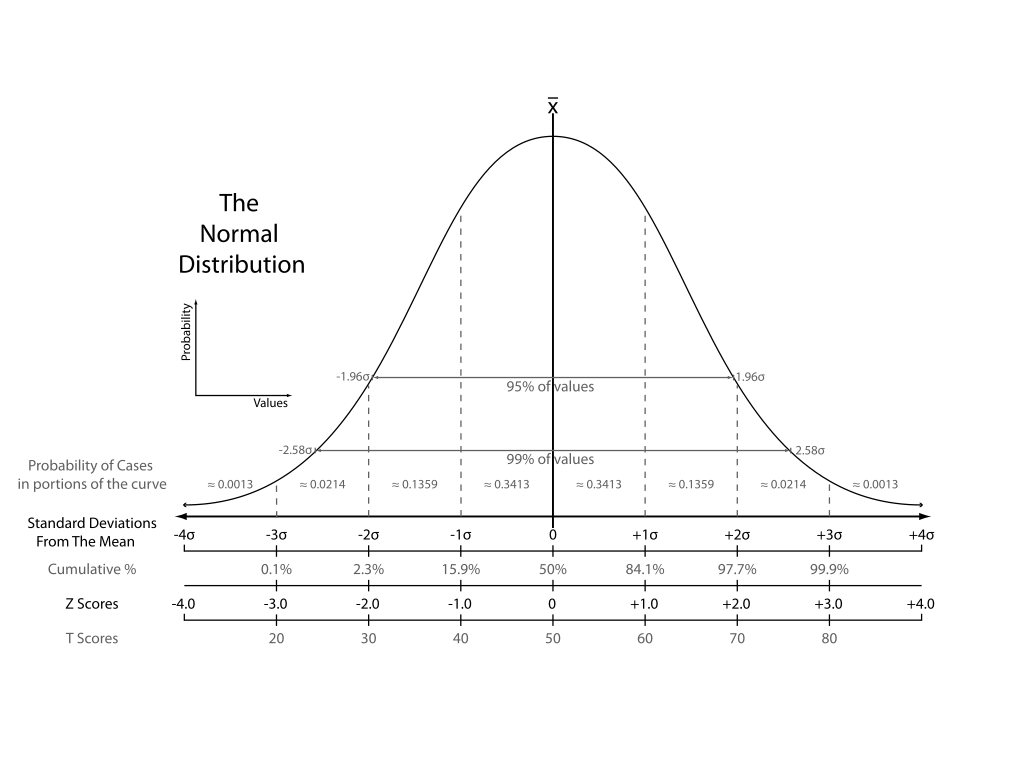
\includegraphics[width=9.48in]{images/normal-dist} 

}

\caption{Distribusi normal}\label{fig:unnamed-chunk-1}
\end{figure}

Berikut adalah rumus \emph{standard error of mean} (\emph{SE}\(\mu\)) adalah..

\[
SE_\mu = \frac{S_y}{\sqrt{n}}
\]

Dimana \emph{S}\textsubscript{y} adalah \textbf{standar deviasi sampel} dan \emph{n} adalah jumlah sampel. Untuk \emph{standard error of proportion}

Menentukan sampel dengan teknik \emph{probability sampling} adalah strategi yang ideal di dunia yang sempurna. Padahal yang lebih sering terjadi, peneliti menghadapi kondisi dimana \emph{probability sampling} tidak dapat dilakukan. Kendala yang paling umum adalah peneliti tidak memiliki informasi yang cukup untuk membuat \emph{sampling frame} sehingga peluang terpilihnya satu unit sampel tidak dapat diketahui. Dalam kondisi ini, peneliti dapat menggunakan \textbf{\emph{non-probability sampling}} dimana sampel ditarik tanpa proses pengacakan. Implikasinya memang tidak menyenangkan - bias dan \emph{sampling error} tidak dapat diestimasi sehingga generalisasi sulit sekali dilakukan.

\textbf{4.1.2 Ragam desain penelitian survei (\emph{cross-sectional}, longitudinal, \emph{cross-lagged panel survey})}

\textbf{4.1.3 \emph{Total survey error}}

\textbf{4.1.4 Metode administrasi survei}

\textbf{4.1.5 Survei opini publik}

\hypertarget{eksperimental}{%
\subsection{4.2 Eksperimental}\label{eksperimental}}

\begin{verbatim}
- Kausalitas versus asosiasi
- Ragam desain eksperimen (*within* dan *between-group design*)
- Validitas internal dan eksternal penelitian eksperimen
- Pendekatan survei eksperimen
\end{verbatim}

\hypertarget{pemrosesan-teks-natural-language-processing-dan-metode-implisit}{%
\subsection{\texorpdfstring{4.3 Pemrosesan teks (\emph{natural language processing}) dan metode implisit}{4.3 Pemrosesan teks (natural language processing) dan metode implisit}}\label{pemrosesan-teks-natural-language-processing-dan-metode-implisit}}

\hypertarget{penelitian-meta-tinjauan-sistematis-dan-meta-analisis}{%
\subsection{4.4 Penelitian meta (tinjauan sistematis dan meta-analisis)}\label{penelitian-meta-tinjauan-sistematis-dan-meta-analisis}}

\begin{verbatim}
- Kelebihan dan fungsi penelitian kumulatif
- Tren penelitian meta dalam perkembangan Psikologi Politik
\end{verbatim}

\hypertarget{penyimpulan-karakter-tokoh-politik-dengan-pendekatan-at-a-distance}{%
\subsection{\texorpdfstring{4.5 Penyimpulan karakter tokoh politik dengan pendekatan \emph{at a distance}}{4.5 Penyimpulan karakter tokoh politik dengan pendekatan at a distance}}\label{penyimpulan-karakter-tokoh-politik-dengan-pendekatan-at-a-distance}}

\hypertarget{pendekatan-interpretif-kualitatif}{%
\subsection{4.6 Pendekatan interpretif (kualitatif)}\label{pendekatan-interpretif-kualitatif}}

\hypertarget{pengujian-hipotesis}{%
\subsection{5. Pengujian hipotesis}\label{pengujian-hipotesis}}

\hypertarget{kesalahan-penarikan-kesimpulan-dalam-paradigma-null-hypothesis-significant-testing}{%
\subsection{\texorpdfstring{5.1 Kesalahan penarikan kesimpulan dalam paradigma \emph{null hypothesis significant testing}}{5.1 Kesalahan penarikan kesimpulan dalam paradigma null hypothesis significant testing}}\label{kesalahan-penarikan-kesimpulan-dalam-paradigma-null-hypothesis-significant-testing}}

\begin{figure}

{\centering 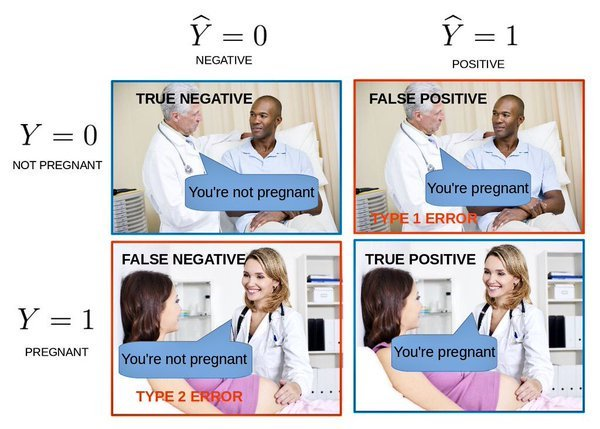
\includegraphics[width=5.56in]{images/confusion-matrix} 

}

\caption{Kesalahan dalam Penarikan Kesimpulan (Inferensi) Sumber: https://dzone.com/articles/understanding-the-confusion-matrix}\label{fig:unnamed-chunk-2}
\end{figure}

\hypertarget{nilai-p-statistical-power-ukuran-efek-effect-size-dan-rentang-kepercayaan-confidence-interval}{%
\subsection{\texorpdfstring{5.2 Nilai p, \emph{statistical power}, ukuran efek (\emph{effect size}), dan rentang kepercayaan (\emph{confidence interval})}{5.2 Nilai p, statistical power, ukuran efek (effect size), dan rentang kepercayaan (confidence interval)}}\label{nilai-p-statistical-power-ukuran-efek-effect-size-dan-rentang-kepercayaan-confidence-interval}}

\hypertarget{revolusi-kredibilitas-coba-ulang-reproducibility-dan-reka-ulang-replicability-dalam-penelitian-psikologi-politik}{%
\subsection{\texorpdfstring{6. Revolusi kredibilitas: Coba-ulang (\emph{reproducibility}) dan reka-ulang (\emph{replicability}) dalam penelitian Psikologi Politik}{6. Revolusi kredibilitas: Coba-ulang (reproducibility) dan reka-ulang (replicability) dalam penelitian Psikologi Politik}}\label{revolusi-kredibilitas-coba-ulang-reproducibility-dan-reka-ulang-replicability-dalam-penelitian-psikologi-politik}}

\begin{figure}

{\centering 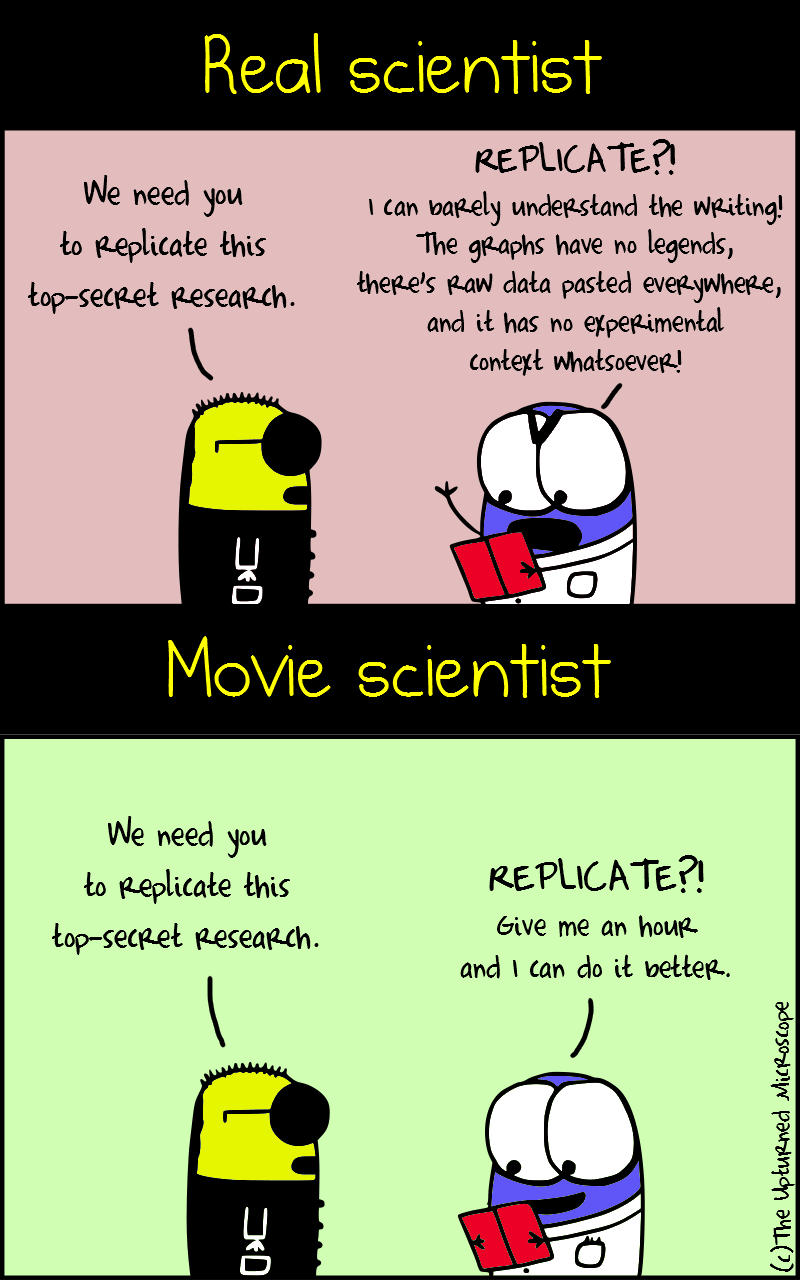
\includegraphics[width=7.42in]{images/replication} 

}

\caption{Reka-ulang Data Penelitian Sumber: https://theupturnedmicroscope.com/}\label{fig:unnamed-chunk-3}
\end{figure}

\hypertarget{krisis-kredibilitas-bias-publikasi-dan-praktik-meneliti-yang-meragukan-questionable-research-practices}{%
\subsection{\texorpdfstring{6.1 Krisis kredibilitas, bias publikasi, dan praktik meneliti yang meragukan (\emph{questionable research practices})}{6.1 Krisis kredibilitas, bias publikasi, dan praktik meneliti yang meragukan (questionable research practices)}}\label{krisis-kredibilitas-bias-publikasi-dan-praktik-meneliti-yang-meragukan-questionable-research-practices}}

\hypertarget{tantangan-dan-peluang-bagi-peneliti-indonesia}{%
\subsection{6.2 Tantangan dan peluang bagi peneliti Indonesia}\label{tantangan-dan-peluang-bagi-peneliti-indonesia}}

\hypertarget{petunjuk-praktis-menjamin-reproduksibilitas-penelitian}{%
\subsection{6.3 Petunjuk praktis menjamin reproduksibilitas penelitian}\label{petunjuk-praktis-menjamin-reproduksibilitas-penelitian}}

\hypertarget{pra-registrasi}{%
\subsection{6.3.1 Pra-registrasi}\label{pra-registrasi}}

\hypertarget{manajemen-data-penelitian-berbasis-kendali-versi-version-control}{%
\subsection{\texorpdfstring{6.3.2 Manajemen data penelitian berbasis kendali versi (\emph{version control})}{6.3.2 Manajemen data penelitian berbasis kendali versi (version control)}}\label{manajemen-data-penelitian-berbasis-kendali-versi-version-control}}

\begin{figure}

{\centering 
\includegraphics[width=12.02in]{images/data-sharing} 

}

\caption{Reka-ulang Data Penelitian Sumber: https://theupturnedmicroscope.com/}\label{fig:unnamed-chunk-4}
\end{figure}

\hypertarget{akses-terbuka}{%
\subsection{6.3.3 Akses terbuka}\label{akses-terbuka}}

\hypertarget{isu-isu-etika-dalam-penelitian-psikologi-politik}{%
\subsection{7. Isu-isu etika dalam penelitian Psikologi Politik}\label{isu-isu-etika-dalam-penelitian-psikologi-politik}}

\hypertarget{anonimitas-dan-kerahasiaan}{%
\subsection{7.1 Anonimitas dan kerahasiaan}\label{anonimitas-dan-kerahasiaan}}

\hypertarget{persetujuan-atas-tindakan-informed-consent}{%
\subsection{\texorpdfstring{7.2 Persetujuan atas tindakan (\emph{informed consent})}{7.2 Persetujuan atas tindakan (informed consent)}}\label{persetujuan-atas-tindakan-informed-consent}}

\hypertarget{transparansi-dan-risiko-pengungkapan-disclosure-risk}{%
\subsection{\texorpdfstring{7.3 Transparansi dan risiko pengungkapan (\emph{disclosure risk})}{7.3 Transparansi dan risiko pengungkapan (disclosure risk)}}\label{transparansi-dan-risiko-pengungkapan-disclosure-risk}}

\newpage

\hypertarget{references}{%
\section{References}\label{references}}

\begingroup
\setlength{\parindent}{-0.5in}
\setlength{\leftskip}{0.5in}

\hypertarget{refs}{}
\leavevmode\hypertarget{ref-bornsteinProcessfocusedModelTest2011}{}%
Bornstein, R. F. (2011). Toward a process-focused model of test score validity: Improving psychological assessment in science and practice. \emph{Psychological Assessment}, \emph{23}(2), 532--544. \url{https://doi.org/10.1037/a0022402}

\leavevmode\hypertarget{ref-choMakingReliabilityReliable2016}{}%
Cho, E. (2016). Making Reliability Reliable: A Systematic Approach to Reliability Coefficients. \emph{Organizational Research Methods}, \emph{19}(4), 651--682. \url{https://doi.org/10.1177/1094428116656239}

\leavevmode\hypertarget{ref-cronbachConstructValidityPsychological1955}{}%
Cronbach, L. J., \& Meehl, P. E. (1955). Construct Validity in Psychological Test. \emph{Psychological Bulletin}, \emph{52}(4), 281--302.

\leavevmode\hypertarget{ref-dienesUnderstandingPsychologyScience2008}{}%
Dienes, Z. (2008). \emph{Understanding psychology as a science}. London: Palgrave Macmillan.

\leavevmode\hypertarget{ref-Duckitt2001}{}%
Duckitt, J. (2001). A dual-process cognitive-motivational theory of ideology and prejudice. In \emph{Advances in experimental social psychology} (Vol. 33, pp. 41--113). \url{https://doi.org/10.1016/S0065-2601(01)80004-6}

\leavevmode\hypertarget{ref-dumenciMultitraitMultimethodAnalysis2000}{}%
Dumenci, L. (2000). Multitrait-Multimethod Analysis. In H. E. Tinsley \& S. D. Brown (Eds.), \emph{Handbook of Applied Multivariate Statistics and Mathematical Modeling} (pp. 583--611). San Diego: Elsevier. \url{https://doi.org/10.1016/B978-0-12-691360-6.X5000-9}

\leavevmode\hypertarget{ref-dunnAlphaOmegaPractical2014}{}%
Dunn, T. J., Baguley, T., \& Brunsden, V. (2014). From alpha to omega: A practical solution to the pervasive problem of internal consistency estimation. \emph{British Journal of Psychology}, \emph{105}(3), 399--412. \url{https://doi.org/10.1111/bjop.12046}

\leavevmode\hypertarget{ref-fowlerSurveyResearchMethods2014}{}%
Fowler, F. J. (2014). \emph{Survey research methods} (Fifth edition). Los Angeles: SAGE.

\leavevmode\hypertarget{ref-friedMeasurementMatters2018}{}%
Fried, E. I., \& Flake, J. K. (2018). Measurement Matters. \emph{APS Observer}, \emph{31}(3).

\leavevmode\hypertarget{ref-hunsleyIncrementalValidityPsychological2003}{}%
Hunsley, J., \& Meyer, G. J. (2003). The Incremental Validity of Psychological Testing and Assessment: Conceptual, Methodological, and Statistical Issues. \emph{Psychological Assessment}, \emph{15}(4), 446--455. \url{https://doi.org/10.1037/1040-3590.15.4.446}

\leavevmode\hypertarget{ref-mairModernPsychometrics2018}{}%
Mair, P. (2018). \emph{Modern Psychometrics with R}. Cham: Springer International Publishing. \url{https://doi.org/10.1007/978-3-319-93177-7}

\leavevmode\hypertarget{ref-marisPsychometricLatentResponse1995}{}%
Maris, E. (1995). Psychometric latent response models. \emph{Psychometrika}, \emph{60}(4), 523--547.

\leavevmode\hypertarget{ref-mcneishThanksCoefficientAlpha2018}{}%
McNeish, D. (2018). Thanks coefficient alpha, we'll take it from here. \emph{Psychological Methods}, \emph{23}(3), 412--433. \url{https://doi.org/10.1037/met0000144}

\leavevmode\hypertarget{ref-messickValidityPsychologicalAssessment1995}{}%
Messick, S. (1995). Validity of Psychological Assessment. \emph{American Psychologist}, 9.

\leavevmode\hypertarget{ref-morlingResearchMethodsPsychology2018}{}%
Morling, B. (2018). \emph{Research Methods in Psychology: Evaluating a World of Information} (3rd ed.). New York, NY: W. W. Norton \& Company, Inc.

\leavevmode\hypertarget{ref-Nosek2015}{}%
Nosek, B. A., Alter, G., Banks, G. C., Borsboom, D., Bowman, S. D., Breckler, S. J., \ldots{} Yarkoni, T. (2015). Promoting an open research culture. \emph{Science}, \emph{348}(6242), 1422--1425. \url{https://doi.org/10.1126/science.aab2374}

\leavevmode\hypertarget{ref-Perezgonzalez2015}{}%
Perezgonzalez, J. D. (2015). Fisher, Neyman-Pearson or NHST? A tutorial for teaching data testing. \emph{Frontiers in Psychology}, \emph{6}(MAR), 1--11. \url{https://doi.org/10.3389/fpsyg.2015.00223}

\leavevmode\hypertarget{ref-petersAlphaOmegaScale2018}{}%
Peters, G. J. Y. (2018). \emph{The alpha and the omega of scale reliability and validity: Why and how to abandon Cronbach's alpha and the route towards more comprehensive assessment of scale quality} (Preprint). PsyArXiv. \url{https://doi.org/10.31234/osf.io/h47fv}

\leavevmode\hypertarget{ref-revelleCoefficientsAlphaBeta2008}{}%
Revelle, W., \& Zinbarg, R. E. (2008). Coefficients Alpha, Beta, Omega, and the glb: Comments on Sijtsma. \emph{Psychometrika}, \emph{74}(1), 145. \url{https://doi.org/10.1007/s11336-008-9102-z}

\leavevmode\hypertarget{ref-ruelPracticeSurveyResearch2016}{}%
Ruel, E. E., Wagner, W. E., \& Gillespie, B. J. (2016). \emph{The practice of survey research: Theory and applications}. Thousand Oaks, CA: Sage Publications, Inc.

\leavevmode\hypertarget{ref-sijtsmaUseMisuseVery2008}{}%
Sijtsma, K. (2008). On the Use, the Misuse, and the Very Limited Usefulness of~Cronbach's Alpha. \emph{Psychometrika}, \emph{74}(1), 107. \url{https://doi.org/10.1007/s11336-008-9101-0}

\leavevmode\hypertarget{ref-skrondalLatentVariableModelling2007}{}%
Skrondal, A., \& Rabe-Hesketh, S. (2007). Latent Variable Modelling: A Survey. \emph{Scandinavian Journal of Statistics}, \emph{34}(4), 712--745. \url{https://doi.org/10.1111/j.1467-9469.2007.00573.x}

\leavevmode\hypertarget{ref-thorntonKarlPopper2019}{}%
Thornton, S. (2019). Karl Popper. In E. N. Zalta (Ed.), \emph{The Stanford Encyclopedia of Philosophy} (Winter 2019). Metaphysics Research Lab, Stanford University.

\leavevmode\hypertarget{ref-wyndTwoQuantitativeApproaches2003}{}%
Wynd, C. A., Schmidt, B., \& Schaefer, M. A. (2003). Two Quantitative Approaches for Estimating Content Validity. \emph{Western Journal of Nursing Research}, \emph{25}(5), 508--518. \url{https://doi.org/10.1177/0193945903252998}

\leavevmode\hypertarget{ref-bornsteinProcessfocusedModelTest2011}{}%
Bornstein, R. F. (2011). Toward a process-focused model of test score validity: Improving psychological assessment in science and practice. \emph{Psychological Assessment}, \emph{23}(2), 532--544. \url{https://doi.org/10.1037/a0022402}

\leavevmode\hypertarget{ref-choMakingReliabilityReliable2016}{}%
Cho, E. (2016). Making Reliability Reliable: A Systematic Approach to Reliability Coefficients. \emph{Organizational Research Methods}, \emph{19}(4), 651--682. \url{https://doi.org/10.1177/1094428116656239}

\leavevmode\hypertarget{ref-cronbachConstructValidityPsychological1955}{}%
Cronbach, L. J., \& Meehl, P. E. (1955). Construct Validity in Psychological Test. \emph{Psychological Bulletin}, \emph{52}(4), 281--302.

\leavevmode\hypertarget{ref-dienesUnderstandingPsychologyScience2008}{}%
Dienes, Z. (2008). \emph{Understanding psychology as a science}. London: Palgrave Macmillan.

\leavevmode\hypertarget{ref-Duckitt2001}{}%
Duckitt, J. (2001). A dual-process cognitive-motivational theory of ideology and prejudice. In \emph{Advances in experimental social psychology} (Vol. 33, pp. 41--113). \url{https://doi.org/10.1016/S0065-2601(01)80004-6}

\leavevmode\hypertarget{ref-dumenciMultitraitMultimethodAnalysis2000}{}%
Dumenci, L. (2000). Multitrait-Multimethod Analysis. In H. E. Tinsley \& S. D. Brown (Eds.), \emph{Handbook of Applied Multivariate Statistics and Mathematical Modeling} (pp. 583--611). San Diego: Elsevier. \url{https://doi.org/10.1016/B978-0-12-691360-6.X5000-9}

\leavevmode\hypertarget{ref-dunnAlphaOmegaPractical2014}{}%
Dunn, T. J., Baguley, T., \& Brunsden, V. (2014). From alpha to omega: A practical solution to the pervasive problem of internal consistency estimation. \emph{British Journal of Psychology}, \emph{105}(3), 399--412. \url{https://doi.org/10.1111/bjop.12046}

\leavevmode\hypertarget{ref-fowlerSurveyResearchMethods2014}{}%
Fowler, F. J. (2014). \emph{Survey research methods} (Fifth edition). Los Angeles: SAGE.

\leavevmode\hypertarget{ref-friedMeasurementMatters2018}{}%
Fried, E. I., \& Flake, J. K. (2018). Measurement Matters. \emph{APS Observer}, \emph{31}(3).

\leavevmode\hypertarget{ref-hunsleyIncrementalValidityPsychological2003}{}%
Hunsley, J., \& Meyer, G. J. (2003). The Incremental Validity of Psychological Testing and Assessment: Conceptual, Methodological, and Statistical Issues. \emph{Psychological Assessment}, \emph{15}(4), 446--455. \url{https://doi.org/10.1037/1040-3590.15.4.446}

\leavevmode\hypertarget{ref-mairModernPsychometrics2018}{}%
Mair, P. (2018). \emph{Modern Psychometrics with R}. Cham: Springer International Publishing. \url{https://doi.org/10.1007/978-3-319-93177-7}

\leavevmode\hypertarget{ref-marisPsychometricLatentResponse1995}{}%
Maris, E. (1995). Psychometric latent response models. \emph{Psychometrika}, \emph{60}(4), 523--547.

\leavevmode\hypertarget{ref-mcneishThanksCoefficientAlpha2018}{}%
McNeish, D. (2018). Thanks coefficient alpha, we'll take it from here. \emph{Psychological Methods}, \emph{23}(3), 412--433. \url{https://doi.org/10.1037/met0000144}

\leavevmode\hypertarget{ref-messickValidityPsychologicalAssessment1995}{}%
Messick, S. (1995). Validity of Psychological Assessment. \emph{American Psychologist}, 9.

\leavevmode\hypertarget{ref-morlingResearchMethodsPsychology2018}{}%
Morling, B. (2018). \emph{Research Methods in Psychology: Evaluating a World of Information} (3rd ed.). New York, NY: W. W. Norton \& Company, Inc.

\leavevmode\hypertarget{ref-Nosek2015}{}%
Nosek, B. A., Alter, G., Banks, G. C., Borsboom, D., Bowman, S. D., Breckler, S. J., \ldots{} Yarkoni, T. (2015). Promoting an open research culture. \emph{Science}, \emph{348}(6242), 1422--1425. \url{https://doi.org/10.1126/science.aab2374}

\leavevmode\hypertarget{ref-Perezgonzalez2015}{}%
Perezgonzalez, J. D. (2015). Fisher, Neyman-Pearson or NHST? A tutorial for teaching data testing. \emph{Frontiers in Psychology}, \emph{6}(MAR), 1--11. \url{https://doi.org/10.3389/fpsyg.2015.00223}

\leavevmode\hypertarget{ref-petersAlphaOmegaScale2018}{}%
Peters, G. J. Y. (2018). \emph{The alpha and the omega of scale reliability and validity: Why and how to abandon Cronbach's alpha and the route towards more comprehensive assessment of scale quality} (Preprint). PsyArXiv. \url{https://doi.org/10.31234/osf.io/h47fv}

\leavevmode\hypertarget{ref-revelleCoefficientsAlphaBeta2008}{}%
Revelle, W., \& Zinbarg, R. E. (2008). Coefficients Alpha, Beta, Omega, and the glb: Comments on Sijtsma. \emph{Psychometrika}, \emph{74}(1), 145. \url{https://doi.org/10.1007/s11336-008-9102-z}

\leavevmode\hypertarget{ref-ruelPracticeSurveyResearch2016}{}%
Ruel, E. E., Wagner, W. E., \& Gillespie, B. J. (2016). \emph{The practice of survey research: Theory and applications}. Thousand Oaks, CA: Sage Publications, Inc.

\leavevmode\hypertarget{ref-sijtsmaUseMisuseVery2008}{}%
Sijtsma, K. (2008). On the Use, the Misuse, and the Very Limited Usefulness of~Cronbach's Alpha. \emph{Psychometrika}, \emph{74}(1), 107. \url{https://doi.org/10.1007/s11336-008-9101-0}

\leavevmode\hypertarget{ref-skrondalLatentVariableModelling2007}{}%
Skrondal, A., \& Rabe-Hesketh, S. (2007). Latent Variable Modelling: A Survey. \emph{Scandinavian Journal of Statistics}, \emph{34}(4), 712--745. \url{https://doi.org/10.1111/j.1467-9469.2007.00573.x}

\leavevmode\hypertarget{ref-thorntonKarlPopper2019}{}%
Thornton, S. (2019). Karl Popper. In E. N. Zalta (Ed.), \emph{The Stanford Encyclopedia of Philosophy} (Winter 2019). Metaphysics Research Lab, Stanford University.

\leavevmode\hypertarget{ref-wyndTwoQuantitativeApproaches2003}{}%
Wynd, C. A., Schmidt, B., \& Schaefer, M. A. (2003). Two Quantitative Approaches for Estimating Content Validity. \emph{Western Journal of Nursing Research}, \emph{25}(5), 508--518. \url{https://doi.org/10.1177/0193945903252998}

\endgroup

\clearpage
\renewcommand{\listfigurename}{Figure captions}


\end{document}
